% TikZ 2D: arrow styles, path decorations, and Bézier curves
\documentclass{article}
\usepackage{tikz}
\usetikzlibrary{arrows.meta, decorations.pathmorphing, decorations.markings}

\begin{document}
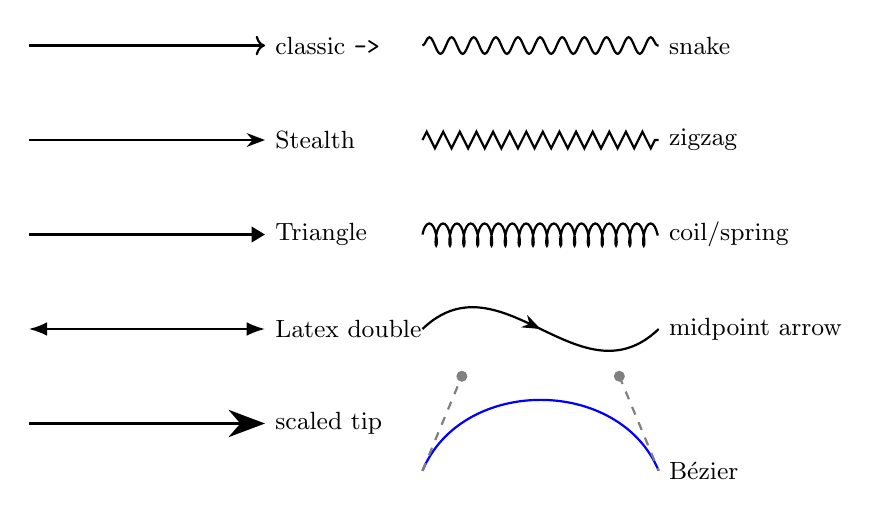
\begin{tikzpicture}[font=\small, line width=0.8pt, y=1.2cm]

  % Classic arrow styles
  \draw[->]           (0,5) -- (3,5) node[right] {classic \texttt{->}};
  \draw[-{Stealth}]   (0,4) -- (3,4) node[right] {Stealth};
  \draw[-{Triangle}]  (0,3) -- (3,3) node[right] {Triangle};
  \draw[{Latex}-{Latex}] (0,2) -- (3,2) node[right] {Latex double};
  \draw[-{Stealth[scale=2]}] (0,1) -- (3,1) node[right] {scaled tip};

  % Decorations
  \draw[decorate, decoration={snake, amplitude=3pt, segment length=8pt}]
    (5,5) -- (8,5) node[right] {snake};
  \draw[decorate, decoration={zigzag, amplitude=3pt, segment length=6pt}]
    (5,4) -- (8,4) node[right] {zigzag};
  \draw[decorate, decoration={coil, aspect=0.3, segment length=5pt, amplitude=4pt}]
    (5,3) -- (8,3) node[right] {coil/spring};

  % Arrow along a curved path using markings
  \draw[postaction={decorate},
        decoration={markings, mark=at position 0.5 with {\arrow{Stealth}}}]
    (5,2) .. controls (6,2.8) and (7,1.2) .. (8,2)
    node[right] {midpoint arrow};

  % Bézier with control points shown
  \draw[blue, thick]
    (5,0.5) .. controls (5.5,1.5) and (7.5,1.5) .. (8,0.5);
  \draw[gray, dashed]
    (5,0.5) -- (5.5,1.5)  (7.5,1.5) -- (8,0.5);
  \fill[gray] (5.5,1.5) circle (2pt) (7.5,1.5) circle (2pt);
  \node[right] at (8,0.5) {Bézier};

\end{tikzpicture}
\end{document}
